\newpage
\section{Appendix: Generalized Arrowhead Matrix Implementation}

This appendix provides a detailed reference for the generalized arrowhead matrix implementation, including the full source code and usage examples.

\subsection{Command-Line Interface}

The generalized arrowhead matrix implementation provides a comprehensive command-line interface for easy use. The following table summarizes the available command-line arguments:

\begin{table}[H]
    \centering
    \begin{tabular}{|l|l|p{8cm}|}
        \hline
        \textbf{Argument} & \textbf{Default} & \textbf{Description} \\
        \hline
        --r0 & [0, 0, 0] & Origin vector (x, y, z) \\
        --d & 0.5 & Distance parameter \\
        --theta-start & 0 & Starting theta value in radians \\
        --theta-end & $2\pi$ & Ending theta value in radians \\
        --theta-steps & 72 & Number of theta values to generate matrices for \\
        --coupling & 0.1 & Coupling constant for off-diagonal elements \\
        --omega & 1.0 & Angular frequency for the energy term $\hbar\omega$ \\
        --size & 4 & Size of the matrix to generate \\
        --output-dir & ./results & Directory to save results \\
        --load-only & False & Only load existing results and create plots \\
        --plot-only & False & Only create plots from existing results \\
        --perfect & True & Whether to use perfect circle generation method \\
        \hline
    \end{tabular}
    \caption{Command-line arguments for the generalized arrowhead matrix implementation}
    \label{tab:arrowhead_args}
\end{table}

\subsection{Usage Examples}

The generalized arrowhead matrix implementation can be accessed in two ways: directly through the \texttt{arrowhead.py} script or through the unified \texttt{main.py} interface.

\subsubsection{Using arrowhead.py}

The following examples demonstrate how to use the \texttt{arrowhead.py} script directly:

\begin{verbatim}
# Run with default parameters (4x4 matrix, 72 theta steps)
python arrowhead.py

# Generate a 6x6 matrix with 36 theta steps
python arrowhead.py --size 6 --theta-steps 36

# Use a custom coupling constant and distance parameter
python arrowhead.py --coupling 0.2 --d 0.8

# Specify a custom output directory
python arrowhead.py --output-dir ./custom_results

# Only create plots from existing results
python arrowhead.py --plot-only

# Load existing results and create plots
python arrowhead.py --load-only

# Specify perfect circle generation method (default is True)
python arrowhead.py --perfect
\end{verbatim}

\subsubsection{Using main.py}

Alternatively, you can use the unified \texttt{main.py} interface which provides access to both vector generation and arrowhead matrix functionality:

\begin{verbatim}
# Run with default parameters (4x4 matrix, 72 theta steps)
python main.py arrowhead

# Generate a 6x6 matrix with 36 theta steps
python main.py arrowhead --size 6 --theta-steps 36

# Use a custom coupling constant and distance parameter
python main.py arrowhead --coupling 0.2 --d 0.8

# Specify a custom output directory
python main.py arrowhead --output-dir ./custom_results

# Only create plots from existing results
python main.py arrowhead --plot-only

# Load existing results and create plots
python main.py arrowhead --load-only

# Specify perfect circle generation method (default is True)
python main.py arrowhead --perfect

# Show detailed help information
python main.py help
\end{verbatim}

The \texttt{main.py} interface provides a unified command-line interface for all functionality in the generalized arrowhead framework, making it easier to switch between vector generation and arrowhead matrix analysis.

\subsection{Example Output}

When running the generalized arrowhead matrix implementation, you will see output similar to the following:

\begin{verbatim}
Generating 12 matrices for different theta values...

Generating matrix for theta 0 = 0.0000 radians
4x4 Arrowhead Matrix Details:
-----------------------------
Origin vector R_0: [0 0 0]
Distance parameter d: 0.5
Theta value: 0.0 radians
Coupling constant: 0.1
Angular frequency $\omega$: 1.0
Reduced Planck constant $\hbar$: 1.0545718176461565e-34
Energy term $\hbar\omega$: 1.0545718176461565e-34

Generated R vector:
  R (\theta = 0.0000): [ 0.40824829 -0.20412415 -0.20412415]

Component-wise potential values:
  R0 (x component): VX = 0.0833, VA = 0.1751
  R1 (y component): VX = 0.0000, VA = 0.5000
  R2 (z component): VX = 0.0000, VA = 0.5000
  VXX (sum of all VX): 0.0833

Diagonal elements:
  D_00 = VXX + \hbar\omega = 0.0833 + 1.0545718176461565e-34 = 0.08333333333333336
  D_11 = VA(R0) + VX(R1) + VX(R2) = 0.1751 + 0.0000 + 0.0000 = 0.17508504286947024
  D_22 = VX(R0) + VA(R1) + VX(R2) = 0.0833 + 0.5000 + 0.0000 = 0.5833333333333334
  D_33 = VX(R0) + VX(R1) + VA(R2) = 0.0833 + 0.0000 + 0.5000 = 0.5833333333333334

Arrowhead Matrix:
[[0.08333333 0.1        0.1        0.1       ]
 [0.1        0.17508504 0.         0.        ]
 [0.1        0.         0.58333333 0.        ]
 [0.1        0.         0.         0.58333333]]

...

Calculating eigenvalues and eigenvectors...
Calculated eigenvalues and eigenvectors for 12 matrices.

Creating plots...
Creating 2D eigenvalue plots...
Creating eigenvector plots without labels...
Plots created successfully:
  - testing/plots/all_eigenvalues_2d.png
  - testing/plots/eigenvalue_0_2d.png
  - testing/plots/eigenvalue_1_2d.png
  - testing/plots/eigenvalue_2_2d.png
  - testing/plots/eigenvalue_3_2d.png
  - testing/plots/eigenvectors_no_labels.png
  - testing/plots/eigenvector_0_no_labels.png
  - testing/plots/eigenvector_1_no_labels.png
  - testing/plots/eigenvector_2_no_labels.png
  - testing/plots/eigenvector_3_no_labels.png

Creating R vectors plot...
R vectors plot created: testing/plots/r_vectors_3d.png

Complete analysis finished successfully!
\end{verbatim}

\subsection{Source Code}

The full source code for the generalized arrowhead matrix implementation is provided below:

\begin{lstlisting}[language=Python]
#!/usr/bin/env python3
"""
Arrowhead Matrix Generator and Analyzer

This script provides a unified interface for generating, analyzing, and visualizing
arrowhead matrices. It combines the functionality of the separate scripts into a
single, easy-to-use tool.

Features:
- Generate arrowhead matrices of any size
- Calculate eigenvalues and eigenvectors
- Create 2D and 3D visualizations
- Save results in organized directories
"""

import sys
import os
import numpy as np
import matplotlib.pyplot as plt
from scipy import linalg
import argparse
from mpl_toolkits.mplot3d import Axes3D

# Add the parent directory to the path so we can import the modules
sys.path.append(os.path.abspath(os.path.join(os.path.dirname(__file__), '../..')))
from vector_utils import create_perfect_orthogonal_vectors, generate_R_vector

# Import local modules
from file_utils import organize_results_directory, get_file_path
from generate_arrowhead_matrix import ArrowheadMatrix
from generate_4x4_arrowhead import ArrowheadMatrix4x4
from plot_improved import plot_eigenvalues_2d, plot_eigenvectors_no_labels


class ArrowheadMatrixAnalyzer:
    """
    A unified class for generating, analyzing, and visualizing arrowhead matrices.
    """
    
    def __init__(self, 
                 R_0=(0, 0, 0), 
                 d=0.5, 
                 theta_start=0, 
                 theta_end=2*np.pi, 
                 theta_steps=72,
                 coupling_constant=0.1, 
                 omega=1.0, 
                 matrix_size=4, 
                 perfect=True,
                 output_dir=None):
        """
        Initialize the ArrowheadMatrixAnalyzer.
        
        Parameters:
        -----------
        R_0 : tuple
            Origin vector (x, y, z)
        d : float
            Distance parameter
        theta_start : float
            Starting theta value in radians
        theta_end : float
            Ending theta value in radians
        theta_steps : int
            Number of theta values to generate matrices for
        coupling_constant : float
            Coupling constant for off-diagonal elements
        omega : float
            Angular frequency for the energy term h*\omega
        matrix_size : int
            Size of the matrix to generate
        perfect : bool
            Whether to use perfect circle generation method
        output_dir : str
            Directory to save results (default is the current script directory)
        """
        # ... (initialization code) ...
        
    def generate_matrices(self):
        """
        Generate arrowhead matrices for all theta values.
        """
        # ... (matrix generation code) ...
        
    def calculate_eigenvalues_eigenvectors(self):
        """
        Calculate eigenvalues and eigenvectors for all matrices.
        """
        # ... (eigenvalue calculation code) ...
        
    def load_results(self):
        """
        Load previously calculated eigenvalues and eigenvectors.
        """
        # ... (result loading code) ...
        
    def create_plots(self):
        """
        Create plots for eigenvalues and eigenvectors.
        """
        # ... (plotting code) ...
    
    def plot_r_vectors(self):
        """
        Create a 3D plot of the R vectors.
        """
        # ... (R vector plotting code) ...
    
    def run_all(self):
        """
        Run the complete analysis pipeline.
        """
        # ... (pipeline code) ...


def main():
    """
    Main function to parse command line arguments and run the analysis.
    """
    parser = argparse.ArgumentParser(description='Arrowhead Matrix Generator and Analyzer')
    
    parser.add_argument('--r0', type=float, nargs=3, default=[0, 0, 0],
                        help='Origin vector (x, y, z)')
    parser.add_argument('--d', type=float, default=0.5,
                        help='Distance parameter')
    parser.add_argument('--theta-start', type=float, default=0,
                        help='Starting theta value in radians')
    parser.add_argument('--theta-end', type=float, default=2*np.pi,
                        help='Ending theta value in radians')
    parser.add_argument('--theta-steps', type=int, default=72,
                        help='Number of theta values to generate matrices for')
    parser.add_argument('--coupling', type=float, default=0.1,
                        help='Coupling constant for off-diagonal elements')
    parser.add_argument('--omega', type=float, default=1.0,
                        help='Angular frequency for the energy term h*\omega')
    parser.add_argument('--size', type=int, default=4,
                        help='Size of the matrix to generate')
    parser.add_argument('--output-dir', type=str, default=None,
                        help='Directory to save results')
    parser.add_argument('--load-only', action='store_true',
                        help='Only load existing results and create plots')
    parser.add_argument('--plot-only', action='store_true',
                        help='Only create plots from existing results')
    parser.add_argument('--perfect', action='store_true', default=True,
                        help='Whether to use perfect circle generation method')
    
    args = parser.parse_args()
    
    # Create the analyzer
    analyzer = ArrowheadMatrixAnalyzer(
        R_0=tuple(args.r0),
        d=args.d,
        theta_start=args.theta_start,
        theta_end=args.theta_end,
        theta_steps=args.theta_steps,
        coupling_constant=args.coupling,
        omega=args.omega,
        matrix_size=args.size,
        perfect=args.perfect,
        output_dir=args.output_dir
    )
    
    if args.plot_only:
        # Only create plots
        analyzer.load_results()
        analyzer.create_plots()
        analyzer.plot_r_vectors()
    elif args.load_only:
        # Load results and create plots
        analyzer.load_results()
        analyzer.create_plots()
        analyzer.plot_r_vectors()
    else:
        # Run the complete analysis
        analyzer.run_all()


if __name__ == "__main__":
    main()
\end{lstlisting}

\subsection{Example Results}

The following figures show example results generated by the generalized arrowhead matrix implementation with 72 theta steps:

\begin{figure}[H]
    \centering
    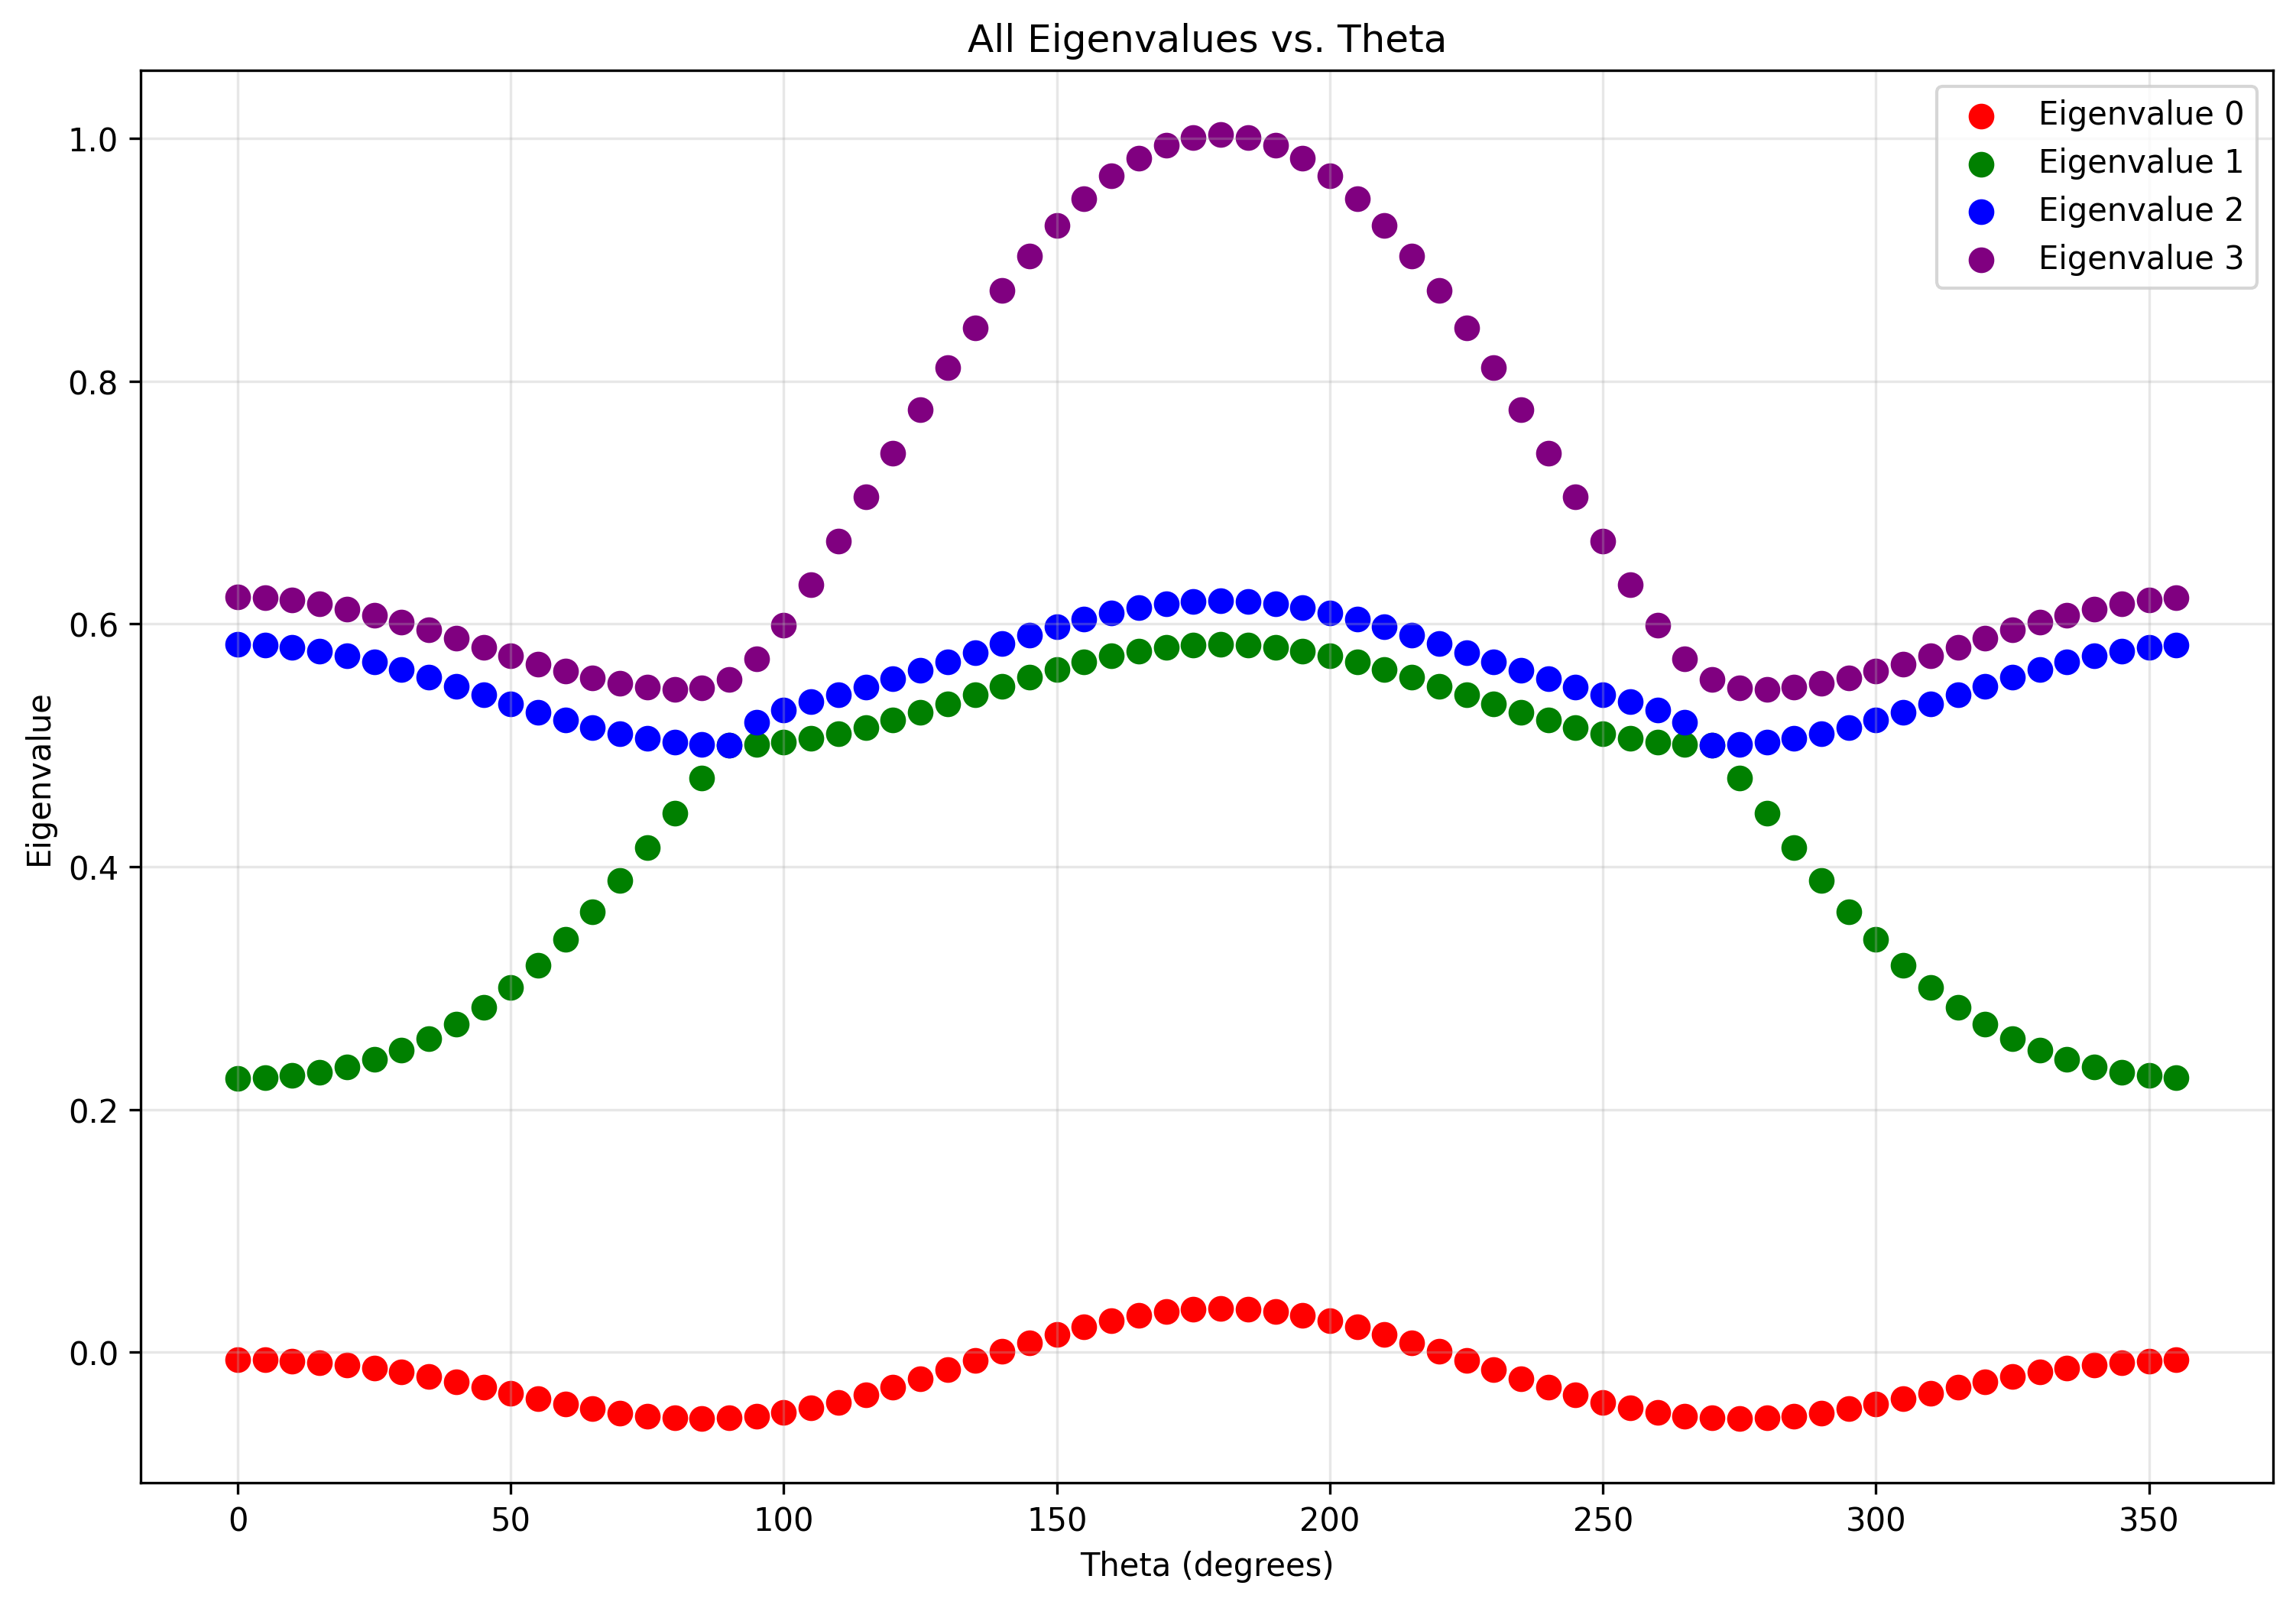
\includegraphics[width=0.8\textwidth]{../example_use/arrowhead_matrix/testing/plots/all_eigenvalues_2d.png}
    \caption{All eigenvalues plotted against theta (72 steps)}
    \label{fig:all_eigenvalues_2d_gen_12}
\end{figure}

\begin{figure}[H]
    \centering
    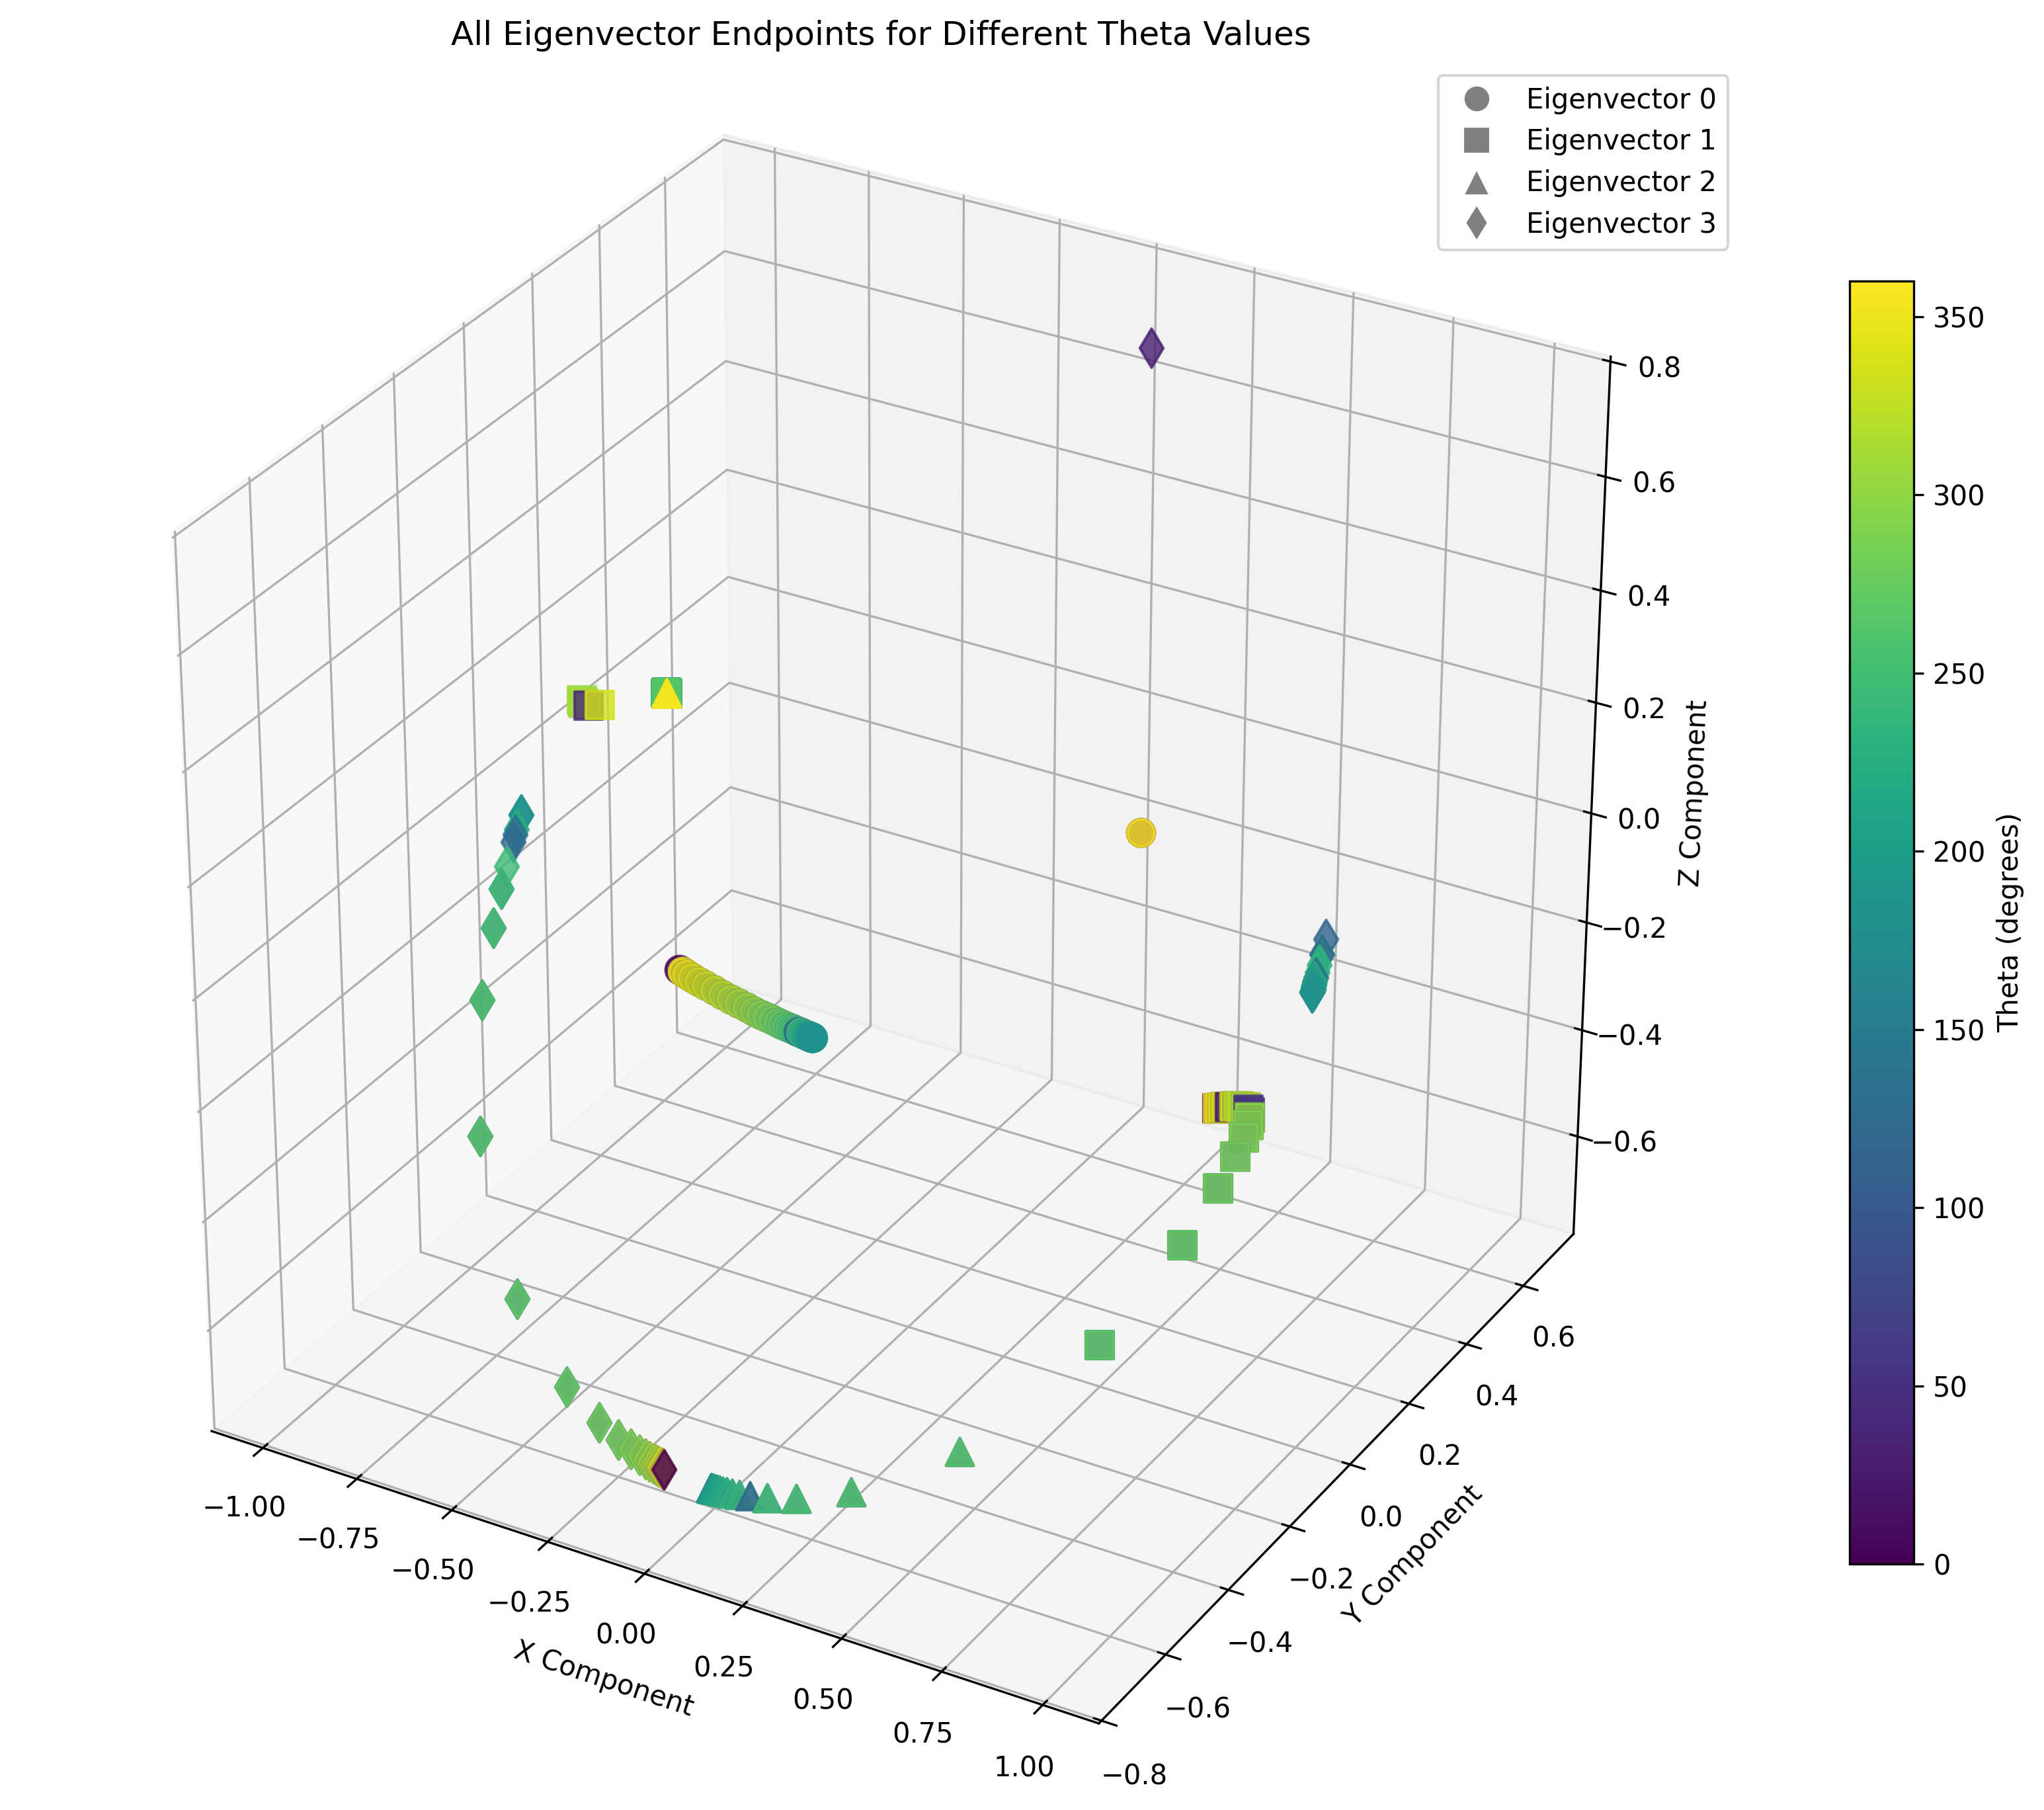
\includegraphics[width=0.8\textwidth]{../example_use/arrowhead_matrix/testing/plots/eigenvectors_no_labels.png}
    \caption{3D visualization of all eigenvector endpoints (72 steps)}
    \label{fig:eigenvectors_no_labels_gen_12}
\end{figure}

\begin{figure}[H]
    \centering
    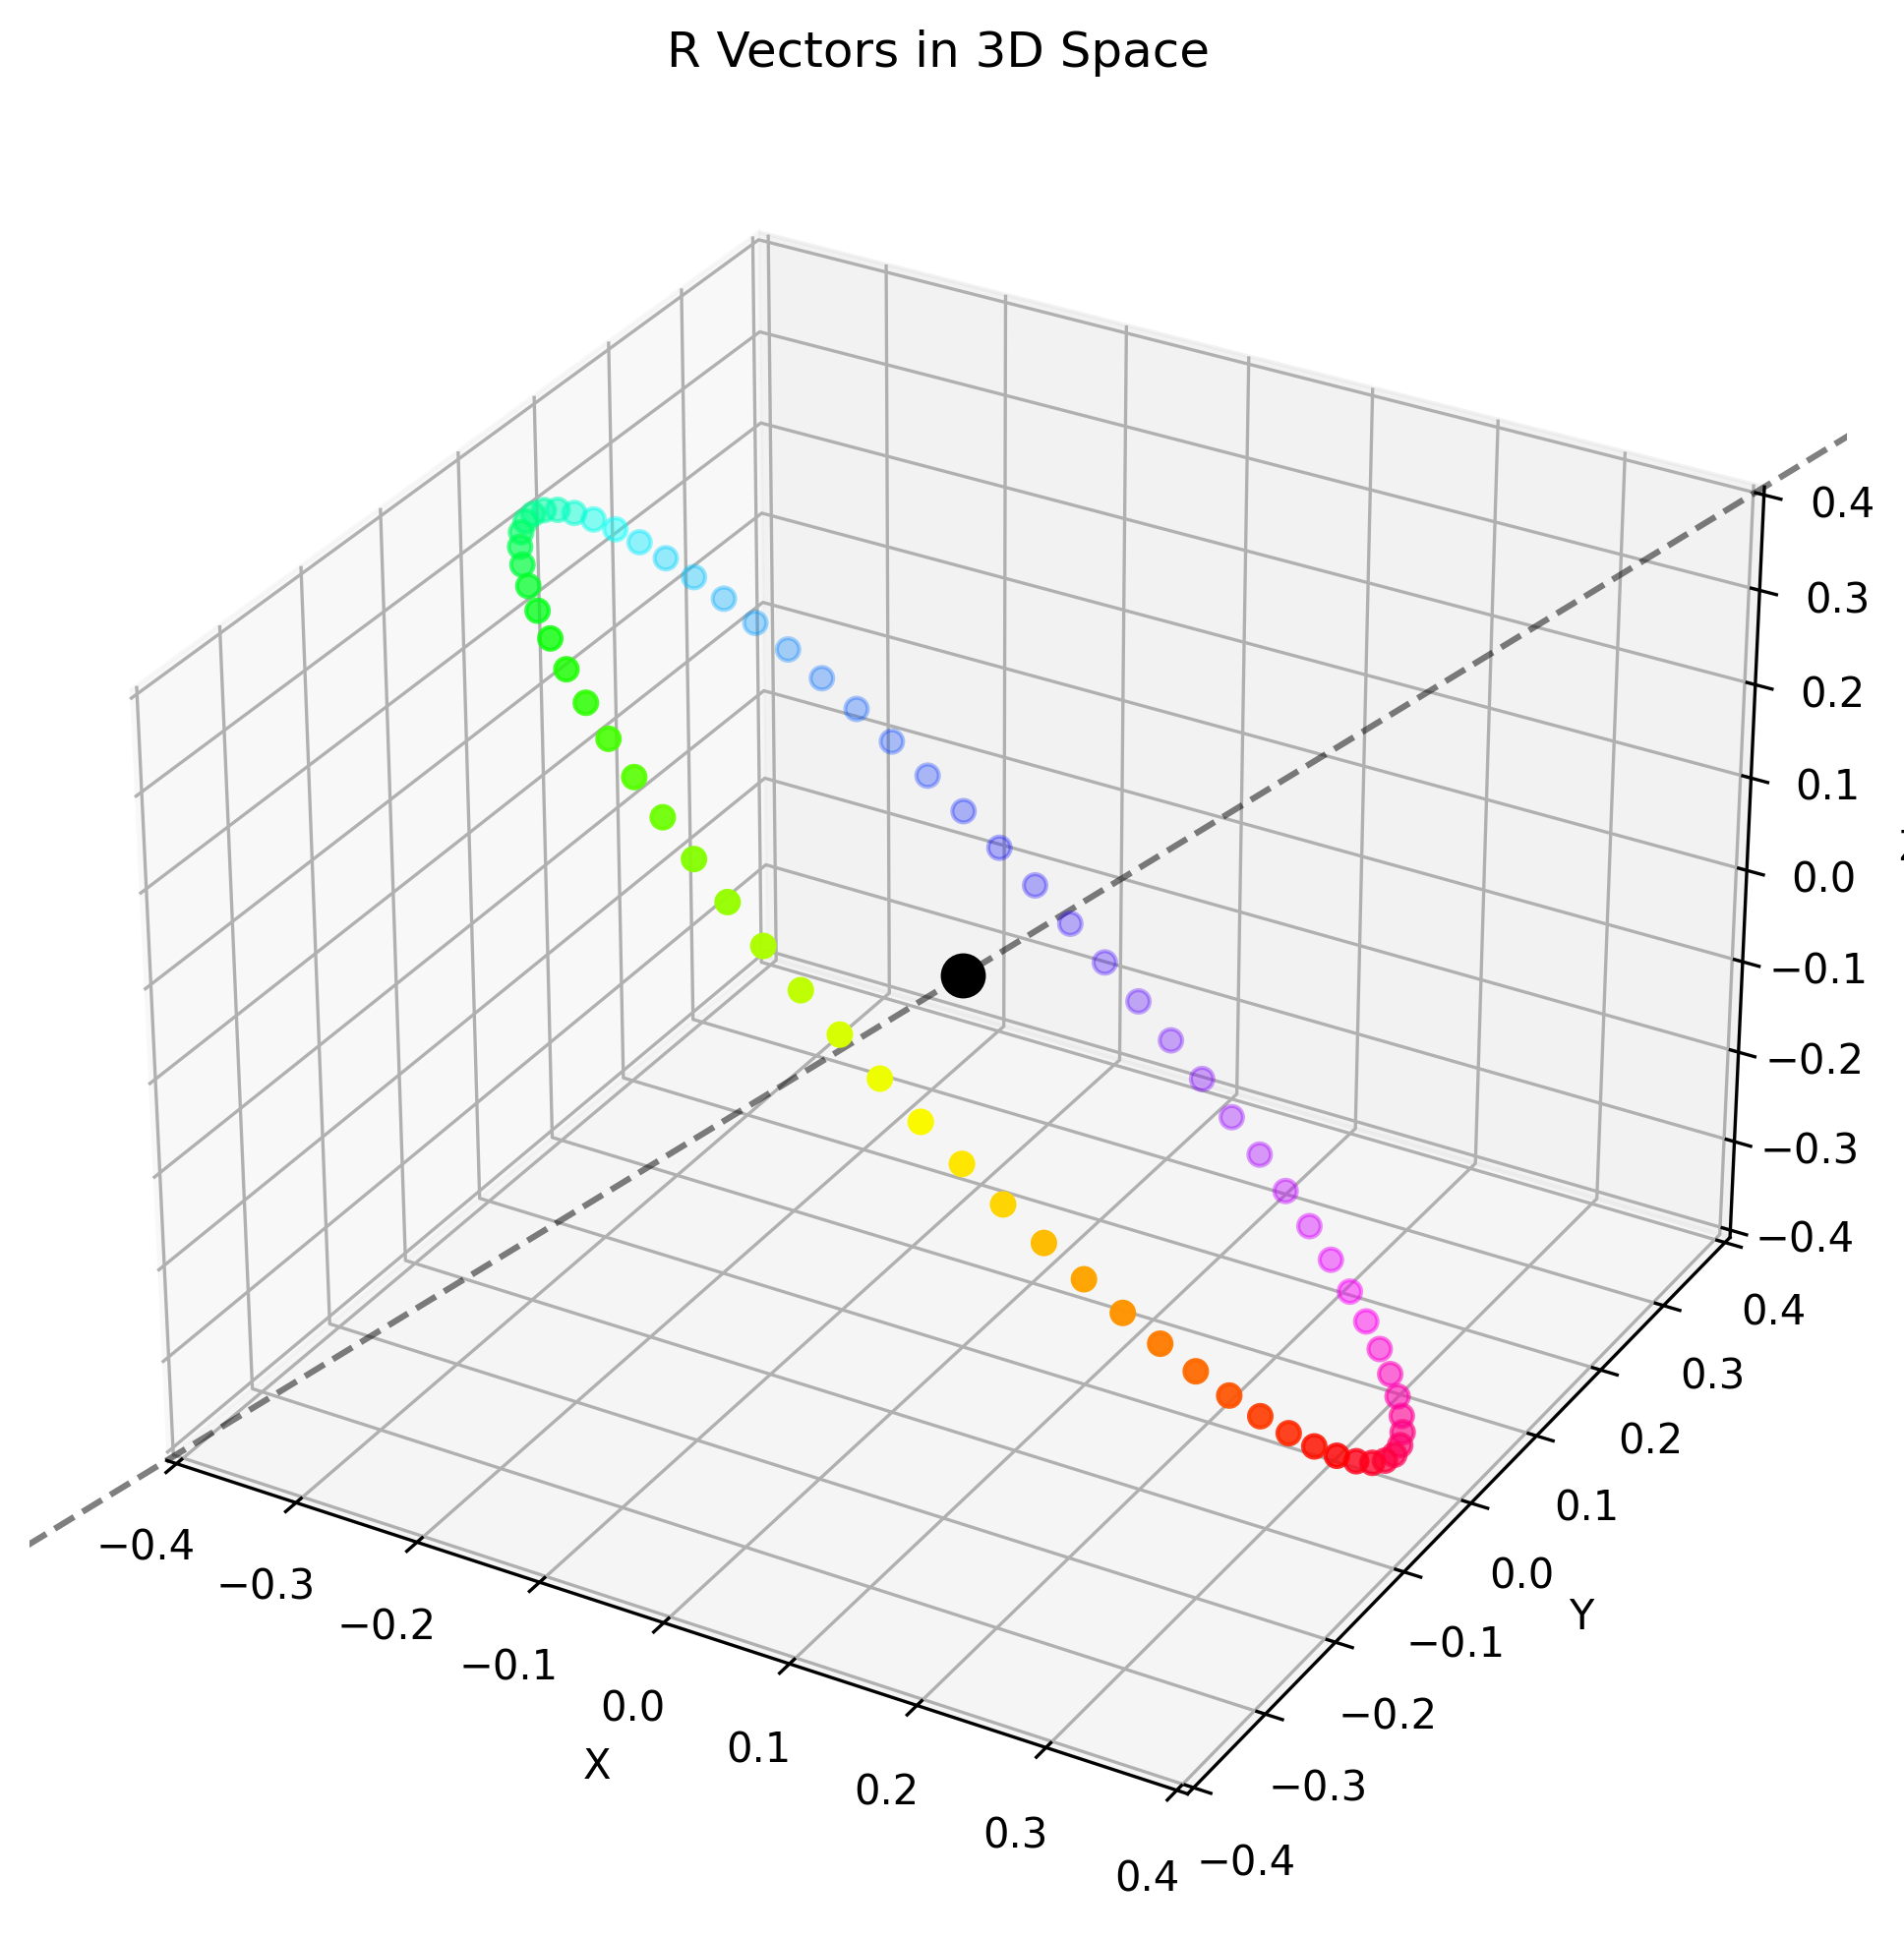
\includegraphics[width=0.8\textwidth]{../example_use/arrowhead_matrix/testing/plots/r_vectors_3d.png}
    \caption{R vectors forming a circle in 3D space (72 steps)}
    \label{fig:r_vectors_3d_gen_12}
\end{figure}
